\section{唯一性与稳定性}
\label{sec:cons-uniqueness}

熵条件排除了前面所有的反例，但这并不等于只剩下一个解。怎样证明同一初值的熵解只有一个？办法是比较两个熵解：证明它们的积分距离不会随时间增大。

\paragraph{距离为什么不增}
先看一个算得出的例子。比较斜坡初值~\eqref{eq:cons-ramp}的解$u$和阶跃初值的解$v$，阶跃位于$x=1/2$，左$1$右$0$。$v$是激波解，位置$x=(1+t)/2$。$u$在$t<1$时由式~\eqref{eq:cons-ramp-solution}给出，$t\geq1$时由式~\eqref{eq:cons-ramp-shock}给出。

$t<1$时，两个解只在区间$(t,1)$上不同。在激波位置$x=(1+t)/2$处，$u$的值是$1/2$，所以差的图像是两个全等的三角形，底为$(1-t)/2$，高为$1/2$。于是
\begin{equation}
  \lVert u(\cdot,t)-v(\cdot,t)\rVert_1=\frac{1-t}{4},\qquad 0\leq t\leq1.
  \label{eq:cons-merge-distance}
\end{equation}

$t=1$时距离为零，此后两个解完全相同，见图~\ref{fig:cons-merge-l1}。距离在减小，而且激波吞掉了两个初值之间的差别。

\begin{BookInlineFigure}
  \centering
  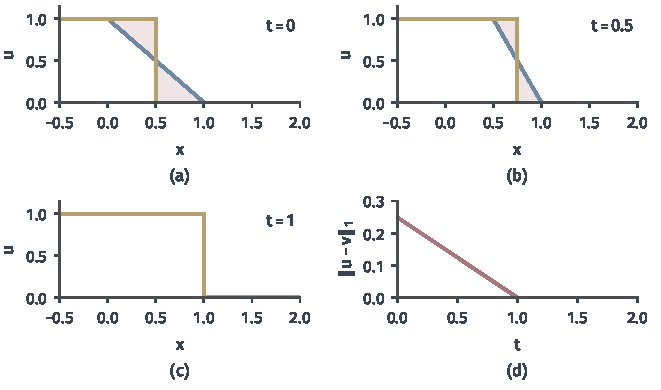
\includegraphics[width=112mm]{figures/06-differential-equations/02-partial-differential-equations/matplotlib/cons-merge-l1/figure.pdf}
  \caption{两个熵解的距离。蓝线是斜坡初值的解，黄线是阶跃初值的解，浅红区域的面积是两者的$L^1$距离。(a)$t=0$。(b)$t=0.5$。(c)$t=1$，两个解重合。(d)距离随时间的变化，$t\leq1$时为$(1-t)/4$，此后为零。}
  \label{fig:cons-merge-l1}
\end{BookInlineFigure}

\paragraph{收缩定理}
一般情形的结论如下。式中的常数$L$是系统中最大的传播速度，它决定了外部区域的影响能传多快。

\begin{theorem}[局部$L^1$收缩]
\label{thm:cons-contraction}
设$F\in C^1(\mathbb{R})$，$u,v$是初值$u_0,v_0\in L^{\infty}(\mathbb{R})$的两个熵解。取$M$使$\lvert u\rvert,\lvert v\rvert\leq M$几乎处处成立，令$L=\max_{\lvert w\rvert\leq M}\lvert F'(w)\rvert$。则对每个$R>0$和几乎处处的$T>0$，
\begin{equation}
  \int_{-R}^{R}\lvert u(x,T)-v(x,T)\rvert\,\mathrm{d}x
  \leq\int_{-R-LT}^{R+LT}\lvert u_0(x)-v_0(x)\rvert\,\mathrm{d}x .
  \label{eq:cons-local-contraction}
\end{equation}
\end{theorem}

图~\ref{fig:cons-cone}是这个不等式的几何含义。$t=T$时区间$[-R,R]$上的差，只由底边$[-R-LT,R+LT]$上的初值差决定，侧边以速度$L$向内收缩。间断可以穿过这个梯形，账依然成立。

\begin{BookInlineFigure}
  \centering
  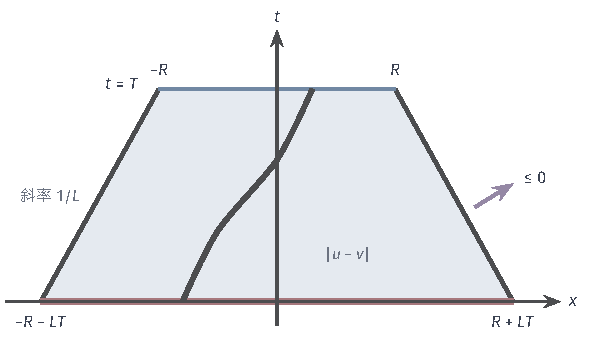
\includegraphics[width=99.8mm]{figures/06-differential-equations/02-partial-differential-equations/tikz/cons-cone/figure.pdf}
  \caption{依赖域梯形。底边（红）是初值差的积分范围，顶边（蓝）是$t=T$时的积分范围，两条侧边（深灰）的速度为$L$。紫色箭头表示穿过侧边的净流量不为正，即差不会从侧边流入。梯形内的深灰曲线是一条可能的间断线。}
  \label{fig:cons-cone}
\end{BookInlineFigure}

证明的难处在于$u$和$v$都不光滑，不能直接相减再求导。若是光滑解，$w=u-v$满足线性输运方程，$\lvert w\rvert$沿特征线的积分不增，结论立刻得到。Kruzhkov的办法是\term{变量加倍}（doubling of variables）：让$u$依赖$(x,t)$，$v$依赖独立的$(y,s)$，在式~\eqref{eq:cons-kruzhkov}中用一个解的值充当另一个解的常数$k$，最后用很窄的权重把$(y,s)$压回$(x,t)$，如图~\ref{fig:cons-doubling}。常数$k$在这里扮演的角色正是Kruzhkov熵的用处：熵不等式对每个$k$成立，$k$就可以取另一个解的值。

\begin{BookInlineFigure}
  \centering
  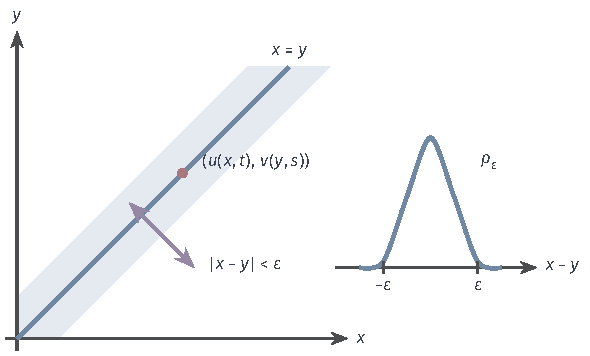
\includegraphics[width=99.9mm]{figures/06-differential-equations/02-partial-differential-equations/tikz/cons-doubling/figure.pdf}
  \caption{变量加倍的示意。左图是$(x,y)$平面（时间变量同理），两个解在两组独立变量上取值，浅蓝带是权重集中的区域，宽度约为$\varepsilon$。右图是横截面上的磨光核$\rho_\varepsilon$。令$\varepsilon\to0$，积分被压回对角线$x=y$。}
  \label{fig:cons-doubling}
\end{BookInlineFigure}

\begin{proof}
记$q(a,b)=\operatorname{sgn}(a-b)(F(a)-F(b))$。它关于$a,b$对称，并且当$\lvert a\rvert,\lvert b\rvert\leq M$时，
\[
  \lvert q(a,b)\rvert\leq L\,\lvert a-b\rvert .
\]

第一步，变量加倍。设$\phi(x,t,y,s)\geq0$是$(\mathbb{R}\times(0,\infty))^2$上的紧支光滑函数。固定$(y,s)$，在式~\eqref{eq:cons-kruzhkov}中对$u$取$k=v(y,s)$，再对$(y,s)$积分。类似地固定$(x,t)$，对$v$取$k=u(x,t)$，对$(x,t)$积分。两式相加，由$q$的对称性，
\[
  \iiiint\Bigl(\lvert u-v\rvert\,(\partial_t\phi+\partial_s\phi)
  +q(u,v)\,(\partial_x\phi+\partial_y\phi)\Bigr)\,\mathrm{d}x\,\mathrm{d}t\,\mathrm{d}y\,\mathrm{d}s\geq0 ,
\]
其中$u=u(x,t)$，$v=v(y,s)$。

第二步，选取测试函数。取非负$\psi\in C_c^{\infty}(\mathbb{R}\times(0,\infty))$和偶的标准磨光核$\rho_\varepsilon$，令
\[
  \phi=\psi\Bigl(\frac{x+y}{2},\frac{t+s}{2}\Bigr)\,
  \rho_\varepsilon\Bigl(\frac{x-y}{2}\Bigr)\,\rho_\varepsilon\Bigl(\frac{t-s}{2}\Bigr).
\]

求$\partial_t\phi+\partial_s\phi$时，$\rho_\varepsilon((t-s)/2)$的两项导数互相抵消，只剩$\psi$对时间的导数，空间变量同样。第一步的不等式化为
\[
  \iiiint\Bigl(\lvert u-v\rvert\,\partial_T\psi+q(u,v)\,\partial_X\psi\Bigr)\rho_\varepsilon\rho_\varepsilon\,\mathrm{d}x\,\mathrm{d}t\,\mathrm{d}y\,\mathrm{d}s\geq0 ,
\]
其中$\partial_T\psi,\partial_X\psi$在中点取值。

第三步，令$\varepsilon\to0$。作变量替换$X=(x+y)/2$，$\xi=(x-y)/2$，$T'=(t+s)/2$，$\tau=(t-s)/2$，Jacobian给出常数因子$4$。$\lvert a-b\rvert$与$q(a,b)$关于$a,b$是Lipschitz的，所以被积函数与其$\xi=\tau=0$时的值之差，被
\[
  C\bigl(\lvert u(X+\xi,T'+\tau)-u(X,T')\rvert+\lvert v(X-\xi,T'-\tau)-v(X,T')\rvert\bigr)
\]
控制。有界函数的平移在$L^1_{\mathrm{loc}}$中连续，这一项的积分在$\varepsilon\to0$时趋于零。于是对所有非负的$\psi$，
\begin{equation}
  \int_0^{\infty}\!\!\int_{\mathbb{R}}\Bigl(\lvert u-v\rvert\,\partial_t\psi+q(u,v)\,\partial_x\psi\Bigr)\,\mathrm{d}x\,\mathrm{d}t\geq0 .
  \label{eq:cons-kato}
\end{equation}

第四步，切出梯形。取$\delta\in(0,R)$和光滑不减函数$H_\delta$，$H_\delta(z)=0$（$z\leq-\delta$），$H_\delta(z)=1$（$z\geq0$）。取$\theta\in C_c^{\infty}(0,T)$，$\theta\geq0$，令
\[
  \psi(x,t)=\theta(t)\,\chi_\delta(x,t),\qquad
  \chi_\delta=1-H_\delta\bigl(\lvert x\rvert+L(t-T)-R\bigr).
\]
在$x=0$附近$H_\delta$的自变量小于$-\delta$，所以$\lvert x\rvert$的不光滑不影响$\psi$的光滑性。

记$H_\delta'$在上述自变量处取值，计算得
\[
  \partial_t\psi=\theta'\chi_\delta-\theta L H_\delta',\qquad
  \partial_x\psi=-\theta\operatorname{sgn}(x)H_\delta' .
\]

代入式~\eqref{eq:cons-kato}，整理后得到
\[
  \int_0^{T}\theta'(t)\int_{\mathbb{R}}\chi_\delta\,\lvert u-v\rvert\,\mathrm{d}x\,\mathrm{d}t
  \geq\iint\theta\,H_\delta'\,\bigl(L\,\lvert u-v\rvert+\operatorname{sgn}(x)\,q(u,v)\bigr)\,\mathrm{d}x\,\mathrm{d}t .
\]

$H_\delta'\geq0$，又由$\lvert q\rvert\leq L\lvert u-v\rvert$，右端非负。这一步是全部证明的关键：侧边的收缩速度$L$压过了流出的通量。

第五步，取极限。令$\delta\to0$，记
\[
  m(t)=\int_{\lvert x\rvert<R+L(T-t)}\lvert u(x,t)-v(x,t)\rvert\,\mathrm{d}x ,
\]
上面的不等式变成$\int_0^T\theta'(t)\,m(t)\,\mathrm{d}t\geq0$对所有非负的$\theta$成立。这说明$m$的弱导数非正，$m$几乎处处等于一个不增函数。

由式~\eqref{eq:cons-entropy-initial}，$t\downarrow0$时$m(t)$的本性极限是$\int_{\lvert x\rvert<R+LT}\lvert u_0-v_0\rvert\,\mathrm{d}x$。于是对几乎处处的$t\in(0,T)$，
\[
  \int_{\lvert x\rvert<R+L(T-t)}\lvert u-v\rvert\,\mathrm{d}x
  \leq\int_{\lvert x\rvert<R+LT}\lvert u_0-v_0\rvert\,\mathrm{d}x .
\]

令$R'=R+L(T-t)$，右端的半径就是$R'+Lt$，这正是要证的形式。让$(R,T)$取遍有理数，两端关于半径连续，所以结论对几乎处处的$t$和所有半径成立。
\end{proof}

证明中的两个地方用到了本章的条件。第一步的$k$可以取任意值，这需要Kruzhkov熵对所有$k$成立，只满足个别几个熵不够。第四步的$\lvert q\rvert\leq L\lvert u-v\rvert$需要$F$在解的取值范围内Lipschitz，这就是通量正则性与解有界的作用。

\paragraph{唯一性、收缩与比较}
把定理~\ref{thm:cons-contraction}用到不同的情形，就得到下面三条结论。比较原理需要把证明中的绝对值换成正部，做法很短，写在证明里。

\begin{theorem}[熵解的唯一性与稳定性]
\label{thm:cons-uniqueness}
在定理~\ref{thm:cons-contraction}的条件下：
\begin{enumerate}
  \item 若$u_0=v_0$几乎处处成立，则$u=v$几乎处处成立，即熵解唯一。
  \item 若$u_0-v_0\in L^1(\mathbb{R})$，则对几乎处处的$t>0$，
  \begin{equation}
    \lVert u(\cdot,t)-v(\cdot,t)\rVert_{1}\leq\lVert u_0-v_0\rVert_{1}.
    \label{eq:cons-l1-contraction}
  \end{equation}
  \item 若$u_0\leq v_0$几乎处处成立，则$u\leq v$几乎处处成立。特别地，$u$的值不超出$u_0$的本性下确界与本性上确界。
\end{enumerate}
\end{theorem}

\begin{proof}
第一条：式~\eqref{eq:cons-local-contraction}的右端为零。

第二条：在式~\eqref{eq:cons-local-contraction}中令$R\to\infty$。

第三条：$(u-k)^{+}$是凸函数，记$\operatorname{sgn}^{+}(z)$在$z>0$时为$1$，否则为$0$，与之配对的熵通量是$\operatorname{sgn}^{+}(u-k)(F(u)-F(k))$；$(k-v)^{+}$也是凸函数，熵通量是$\operatorname{sgn}^{+}(k-v)(F(k)-F(v))$。它们都是$C^2$凸熵的极限，所以各自满足式~\eqref{eq:cons-entropy-ineq}。

在变量加倍中，对$u$用前者并取$k=v(y,s)$，对$v$用后者并取$k=u(x,t)$，两式的被积函数相同，都是$(u-v)^{+}$和$\operatorname{sgn}^{+}(u-v)(F(u)-F(v))$。后者的绝对值同样不超过$L(u-v)^{+}$，所以第二步到第五步逐字照搬，得到
\[
  \int_{-R}^{R}(u-v)^{+}(x,T)\,\mathrm{d}x
  \leq\int_{-R-LT}^{R+LT}(u_0-v_0)^{+}\,\mathrm{d}x .
\]
$u_0\leq v_0$时右端为零，所以$u\leq v$。

常数是方程的熵解，取$v\equiv\operatorname*{ess\,sup}u_0$和$u\equiv\operatorname*{ess\,inf}u_0$作比较，得到值域的结论。
\end{proof}

第二条要求$u_0-v_0$可积，并不要求$u_0$、$v_0$本身可积。第一条和第三条不需要可积性，因为定理~\ref{thm:cons-contraction}是局部的，这正是有限传播速度的好处。阶跃初值不可积，但它和另一个只在有界区间上不同的初值之差可积，式~\eqref{eq:cons-l1-contraction}对它们仍然适用，式~\eqref{eq:cons-merge-distance}就是这样的例子。

存在性没有在这里证明。结论是：$F\in C^1$、$u_0\in L^{\infty}$时，熵解在$\mathbb{R}\times(0,\infty)$上存在且唯一。证明可以由消失黏性或单调差分格式的极限得到，需要一致的有界性和全变差估计，篇幅较长，读者可查阅前面提到的文献。本节的贡献是后半部分：极限至多只有一个，且连续依赖于初值。

\paragraph{收缩的两个推论}
收缩给出了比唯一性更多的信息。设$u_0$的全变差$\mathrm{TV}(u_0)$有限。方程不依赖$x$，所以平移$u(\cdot+h,\cdot)$也是熵解，由式~\eqref{eq:cons-l1-contraction}，
\[
  \lVert u(\cdot+h,t)-u(\cdot,t)\rVert_1\leq\lVert u_0(\cdot+h)-u_0\rVert_1\leq\lvert h\rvert\,\mathrm{TV}(u_0).
\]
除以$\lvert h\rvert$再令$h\to0$，得到$\mathrm{TV}(u(\cdot,t))\leq\mathrm{TV}(u_0)$。熵解不会产生新的振荡。

另一方面，式~\eqref{eq:cons-merge-distance}中的距离在有限时间内变成了零，所以时刻$t=1$的解不能告诉我们初值是斜坡还是阶跃。激波把特征线汇入后就丢掉了它们携带的信息。这个收缩是单向的：时间反演后距离可以增大，所以逆时间的问题不适定。

\paragraph{结论的边界}
这些结论只针对标量方程。系统的情形没有与式~\eqref{eq:cons-l1-contraction}对应的$L^1$收缩，也没有足够多的凸熵来运行变量加倍。已知的系统解理论需要初值全变差较小等附加条件，用的是不同的稳定性泛函。所以本节的结论不能直接移植到守恒律系统。
